\documentclass[aspectratio=1610,t]{beamer}

\usepackage[english]{babel}
\usepackage{hyperref}
\usepackage{minted}
\usepackage{alltt}
\usepackage{amsmath}
\usepackage{graphicx}
\usepackage{xcolor}

\usetheme{metropolis}
\usemintedstyle{xcode}
\definecolor{codebg}{RGB}{247, 247, 246}
\setbeamercolor{background canvas}{bg=white}
\hypersetup{colorlinks,linkcolor=,urlcolor=orange}

\title{Lecture 0: Introduction to the course}
\date{February 16, 2023}
\author{Barinov Denis}
\institute{barinov.diu@gmail.com}

\begin{document}

% ----------------------------------------------------------------- %

\begin{frame}
\maketitle
\end{frame}

% ----------------------------------------------------------------- %

\begin{frame}[c]
\frametitle{Gonna play games?}
\begin{center}
    
\includegraphics[width=\textwidth,height=7cm,keepaspectratio]{images/rust_game.jpg}
\end{center}

\end{frame}

% ----------------------------------------------------------------- %

\begin{frame}[c]
\frametitle{Gonna play games?}
\begin{center}
    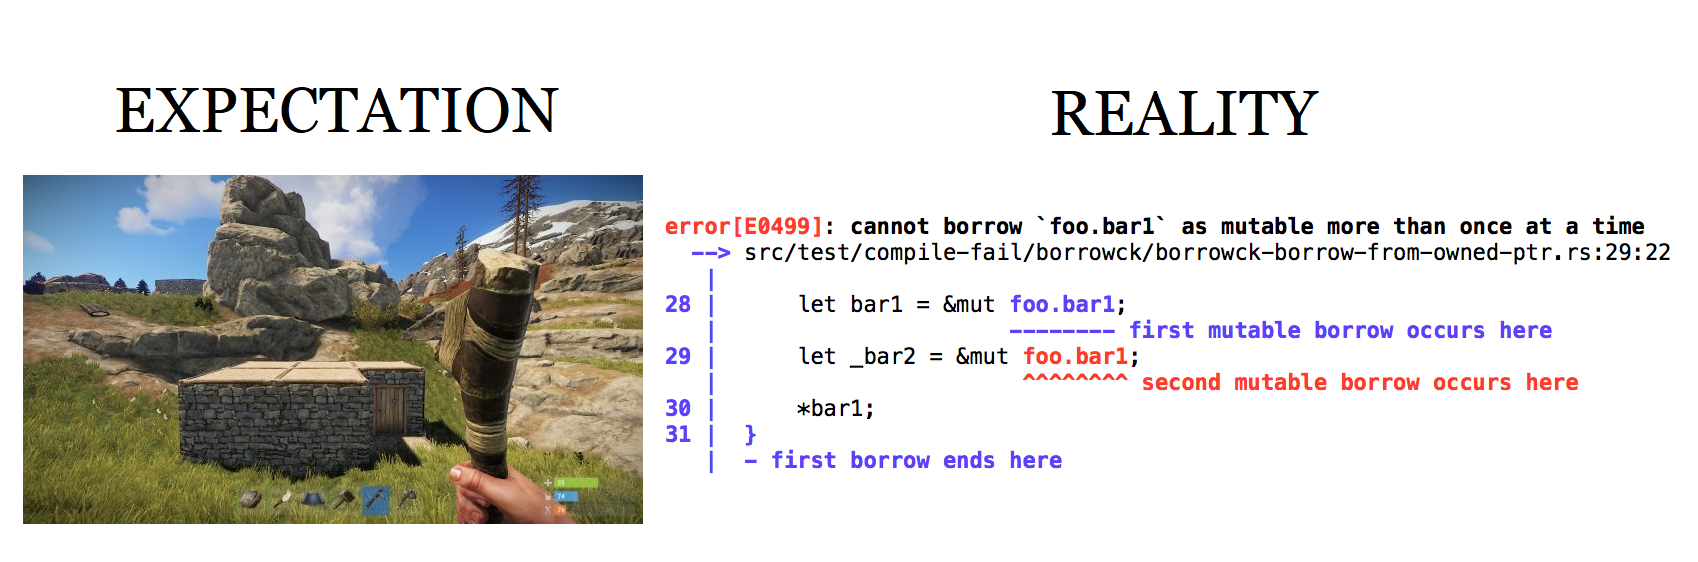
\includegraphics[width=\textwidth,keepaspectratio]{images/borrow_error_mem.png}
\end{center}
\end{frame}

% ----------------------------------------------------------------- %

\begin{frame}[c]
\frametitle{What is this course about?}
The Rust programming language, its basic and advanced features.
\begin{itemize}
    \item Basics: syntax, collections, traits...
    \item Some nightly features, such as trait specialization.
    \item Parallel and concurrent computing.
    \item Metaprogramming.
    \item Tooling around language.
    \item System safety.
\end{itemize}
\end{frame}


% ----------------------------------------------------------------- %

\begin{frame}[c]
\frametitle{Prerequisites}
Nothing special:
\begin{itemize}
    \item Knowledge of C\texttt{++}
    \item Basic understanding of parallel computing and concurrency
    \item Passion for coding
\end{itemize}
\end{frame}

% ----------------------------------------------------------------- %

\begin{frame}[c]
\frametitle{Useful links}
\begin{itemize}
    \item \href{https://www.youtube.com/watch?v=XDv4I3_4Ubs&list=PL4_hYwCyhAvbeLzi699gqMUA4UaPkcdmJ}{Lectures of the previous year}
    \item \href{https://doc.rust-lang.org/book/}{Official Rustbook}
    \item \href{https://doc.rust-lang.org/stable/reference/}{Rust reference}
    \item \href{https://www.youtube.com/c/JonGjengset/featured}{Jon Gjengset}
    \item \href{https://play.rust-lang.org/}{Online IDE}
    \item \dots
\end{itemize}
\end{frame}

% ----------------------------------------------------------------- %

\begin{frame}[c]
\frametitle{How the course will change you}

\begin{center}
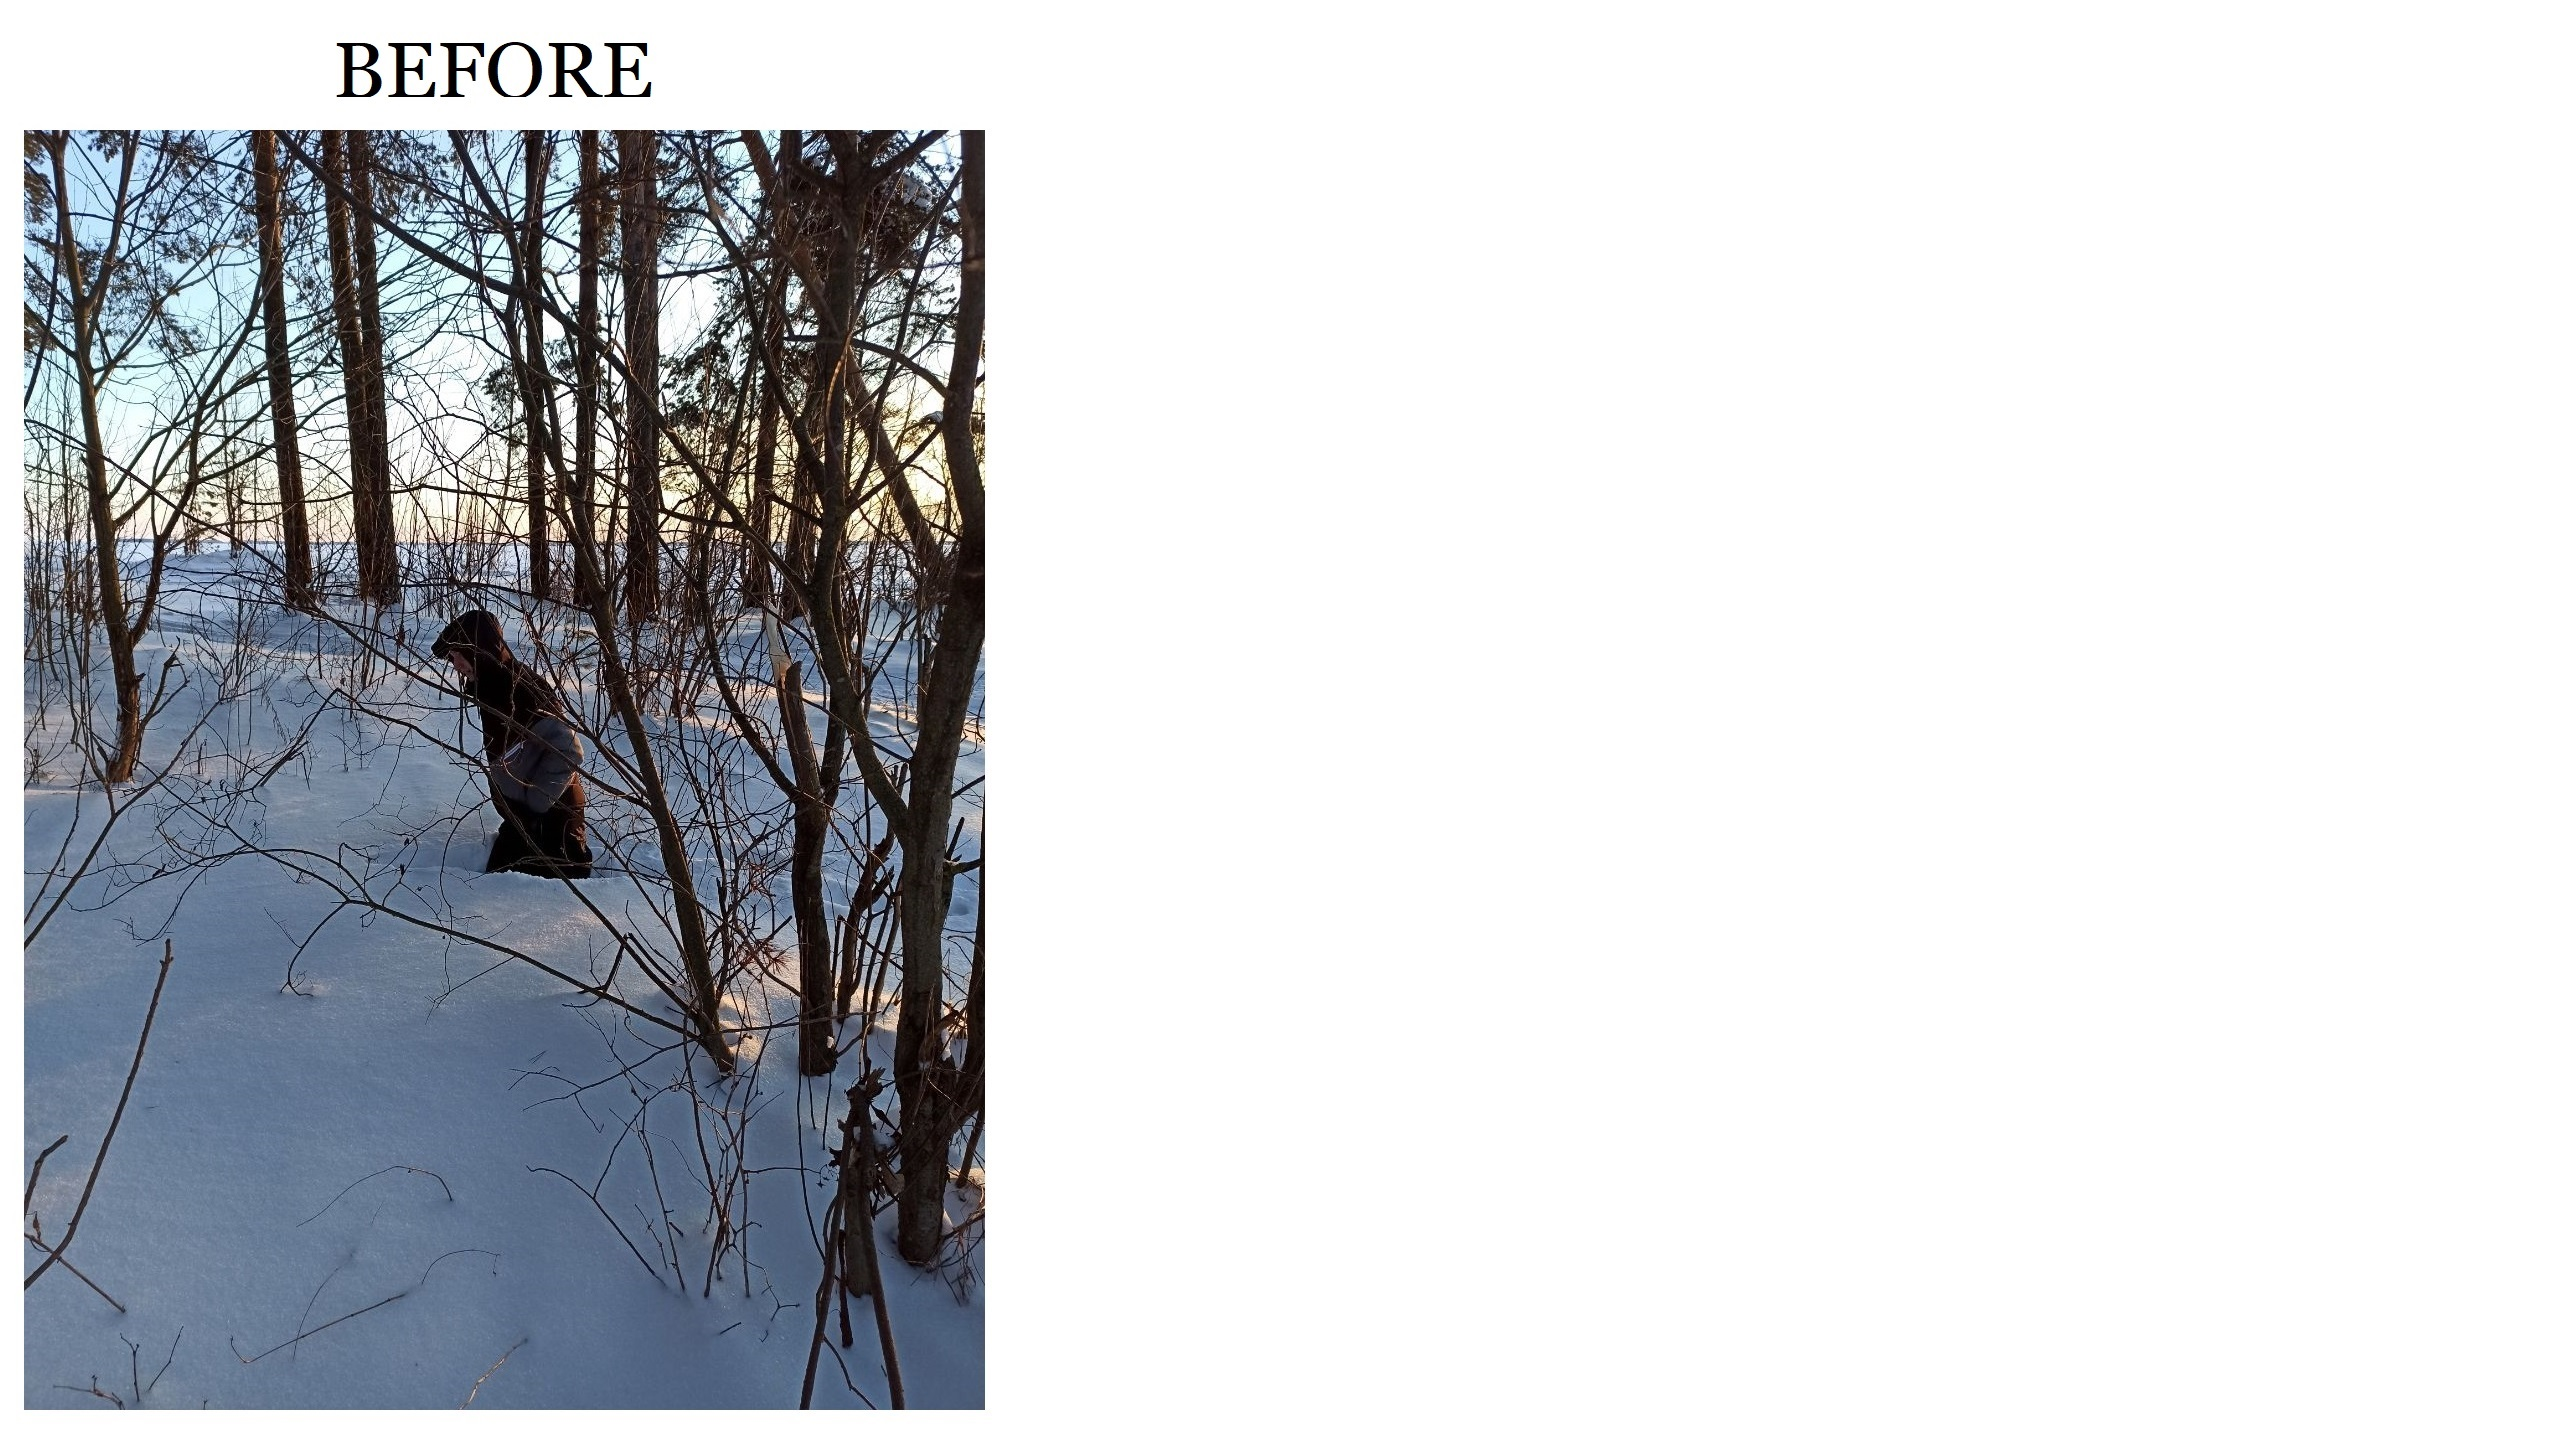
\includegraphics[width=\textwidth,height=7cm,keepaspectratio]{images/me_before.jpg}
\end{center}

\end{frame}

% ----------------------------------------------------------------- %

\begin{frame}[c]
\frametitle{How the course will change you}
\begin{center}
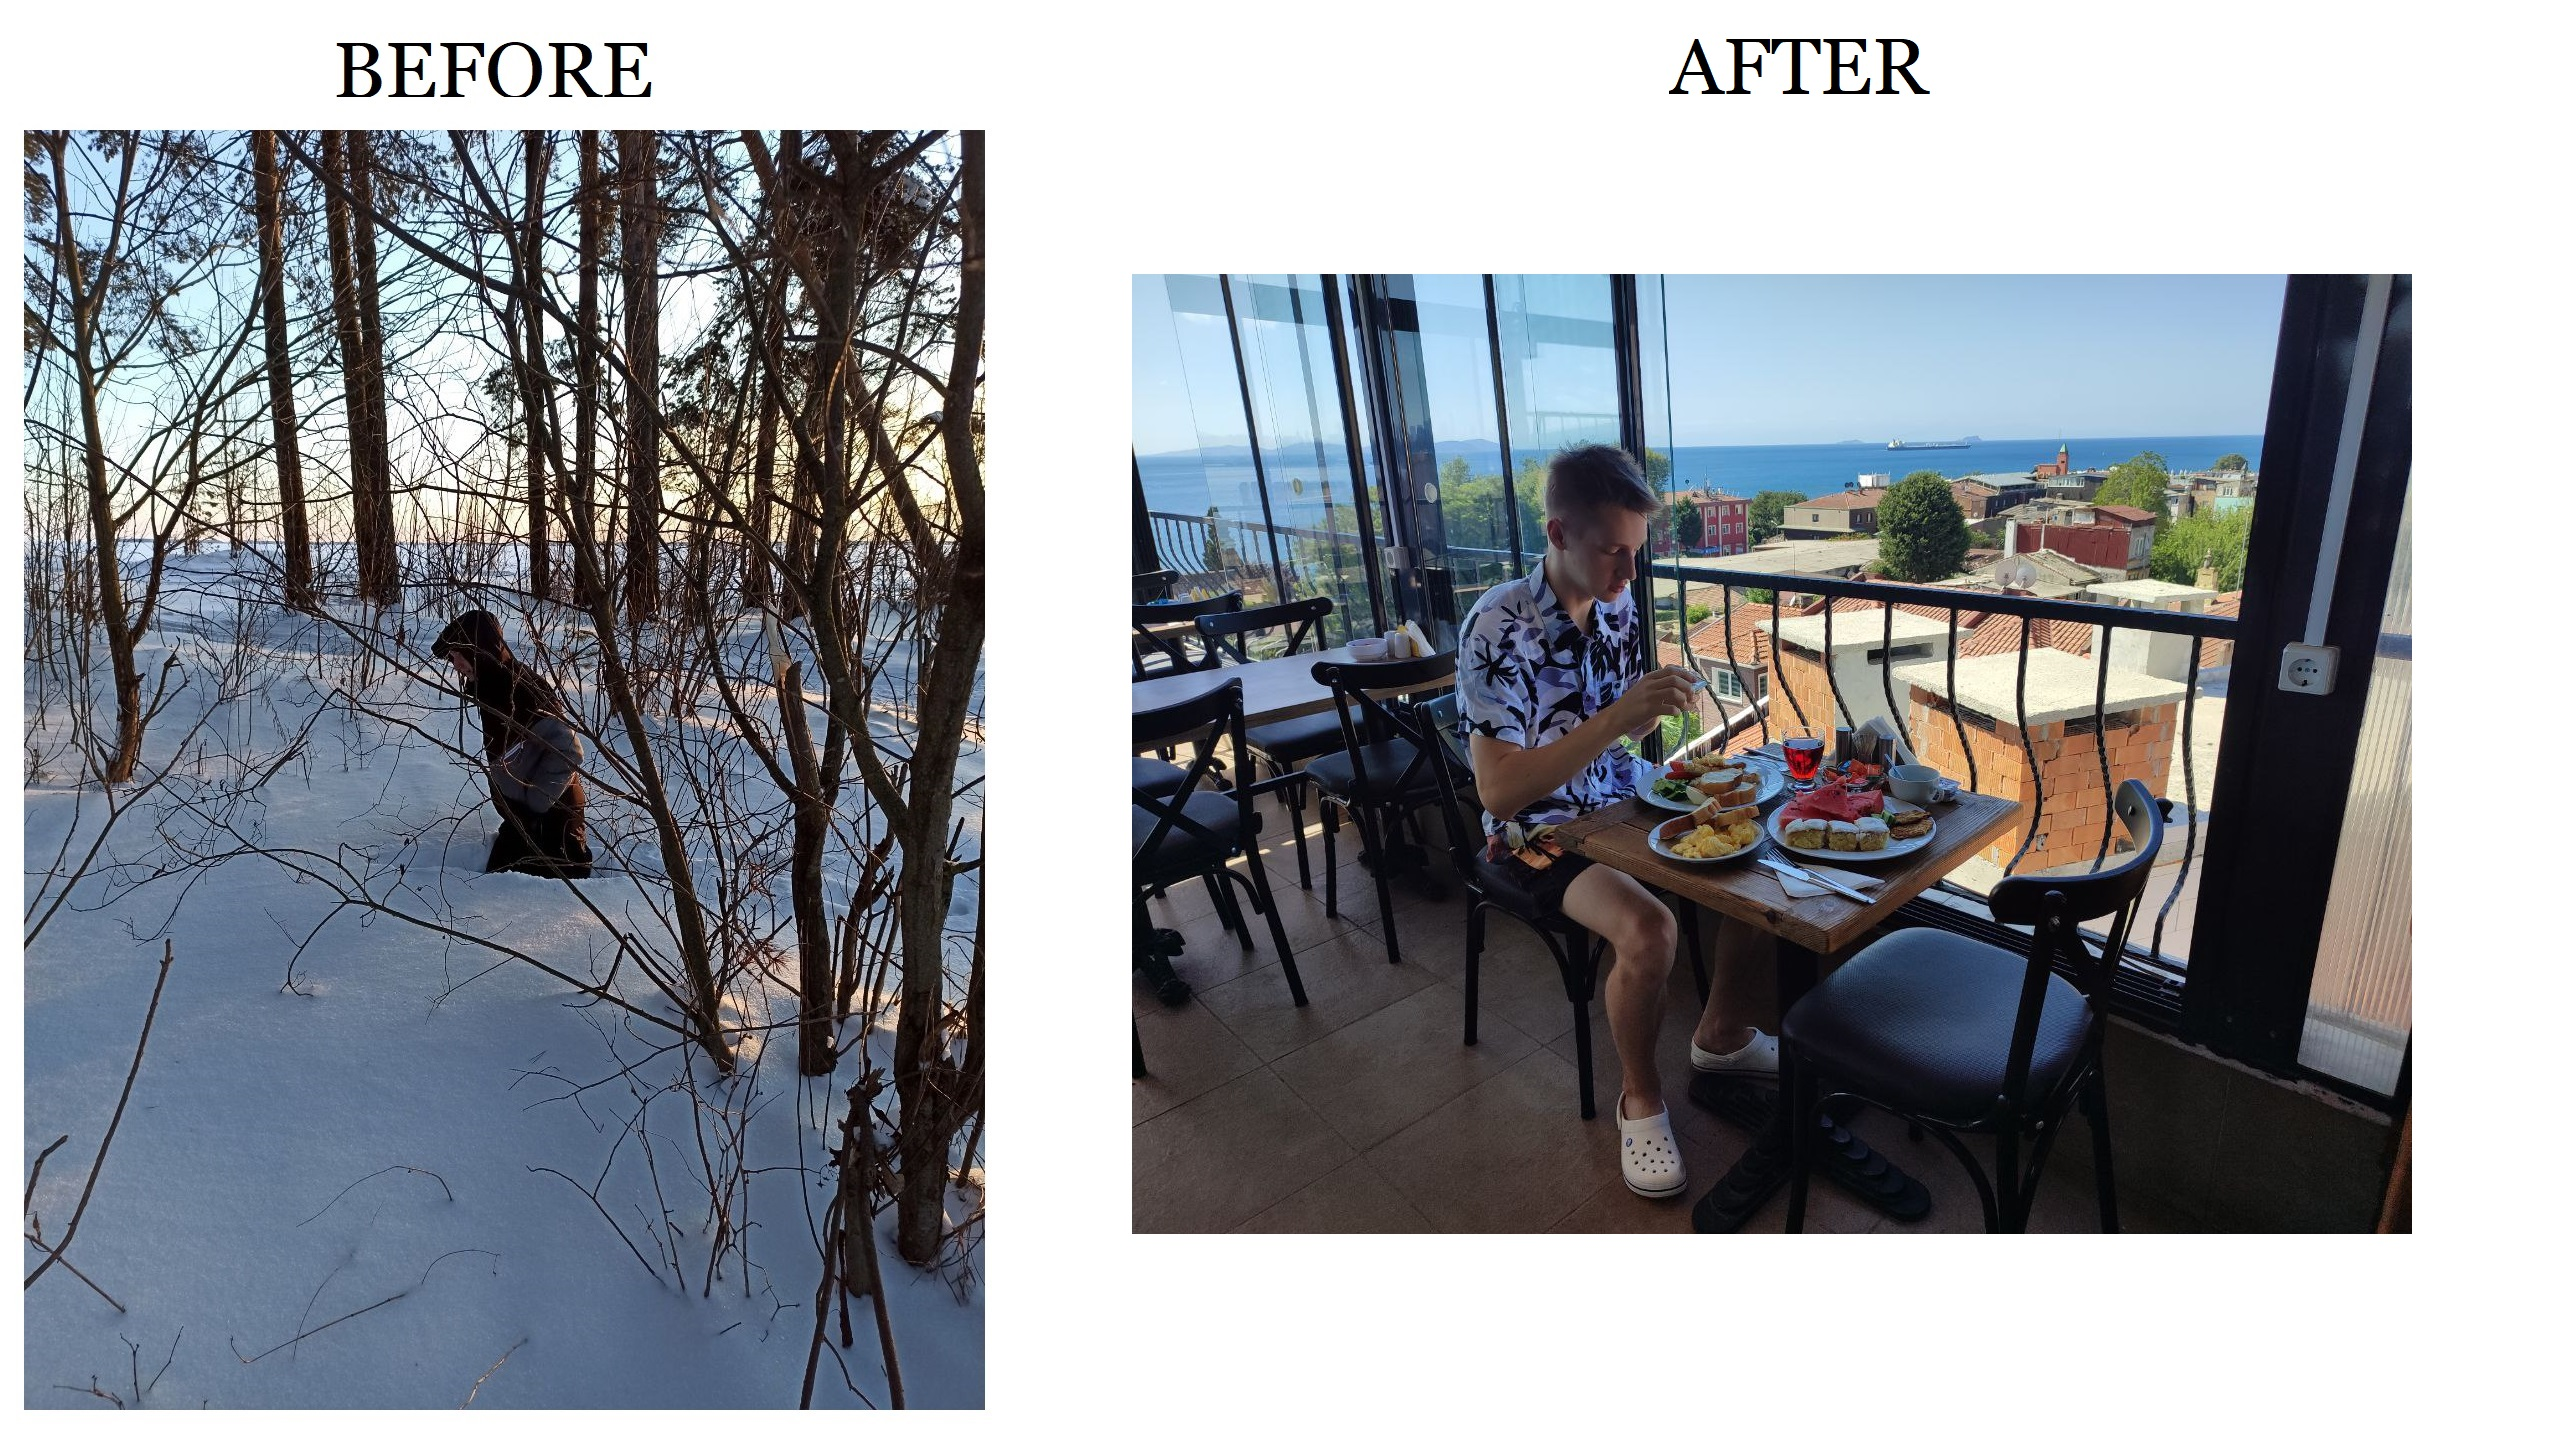
\includegraphics[width=\textwidth,height=7cm,keepaspectratio]{images/me_after.jpg}
\end{center}

\end{frame}

% ----------------------------------------------------------------- %

\begin{frame}
\frametitle{A brief history of Rust\footnote{\href{https://www.youtube.com/watch?v=79PSagCD_AY}{The History of Rust} talk.}}

\begin{enumerate}
    \item \textbf{(2006-2010)} Started at Mozilla by Graydon Hoare as a personal project.
    \item \textbf{(2010-2012)} Rust is now a Mozilla project.
    \begin{itemize}
        \item The team slowly grows allowing Rust to grow faster.
        \item The aim is to make language that can catch critical mistakes before code even compiles.
    \end{itemize}
    \item \textbf{(2012-2014)} Rust improves type system.
    \begin{itemize}
        \item To make the language safe, the team thought they need a garbage collector, but they figured out they don't need it: everything can be done in the level of type system!
        \item Birth of Cargo - the Rust package manager. Influenced by \texttt{ruby} and \texttt{npm}.
    \end{itemize}
    \item \textbf{(2014-present)} Rust grows!
\end{enumerate}
\end{frame}

% ----------------------------------------------------------------- %

\begin{frame}
\frametitle{Who uses Rust?}
\textbf{Google}

\begin{itemize}
    \item \href{https://security.googleblog.com/2021/04/rust-in-linux-kernel.html}{Pushing Rust to Linux Kernel}
    \item \href{https://fuchsia.dev/fuchsia-src/development/languages/rust}{Developing new OS Fuchsia in Rust}\footnote{\href{https://imgur.com/gknVmYk}{Count of lines of code in different languages.}}
    \item \href{https://security.googleblog.com/2021/04/rust-in-android-platform.html}{Enabled support of Rust in Android}
\end{itemize}

\textbf{Meta} 

\begin{itemize}
    \item Mononoke - version control system
    \item Diem - blockchain
    \item Metaverse - virtual reality
\end{itemize}
\end{frame}

% ----------------------------------------------------------------- %

\begin{frame}
\frametitle{Who uses Rust?}
\textbf{Amazon}\footnote{\href{https://aws.amazon.com/blogs/opensource/how-our-aws-rust-team-will-contribute-to-rusts-future-successes/}{How our AWS Rust team will contribute to Rust’s future successes}}

\begin{itemize}
    \item Hired core developers of Tokio (the most popular framework for async)
    \item \href{https://github.com/firecracker-microvm/firecracker}{Firecracker} - open source virtualization technology
    \item \href{https://github.com/bottlerocket-os/bottlerocket}{Bottlerocket OS} - open-source Linux-based operating system meant for hosting containers
    \item \href{https://aws.amazon.com/ec2/nitro/}{Nitro} - compute environments; underlying platform for Amazon EC2
\end{itemize}

\textbf{Microsoft}

\begin{itemize}
    \item \href{https://msrc-blog.microsoft.com/2019/11/07/using-rust-in-windows/}{Rewrited Windows component in Rust}
    \item \href{https://github.com/microsoft/windows-rs}{Official Rust WinAPI wrapper}
\end{itemize}
\end{frame}

% ----------------------------------------------------------------- %

\begin{frame}
\frametitle{Who uses Rust?}
\href{https://discord.com/blog/why-discord-is-switching-from-go-to-rust}{Why Discord is swithing from Go to Rust?}

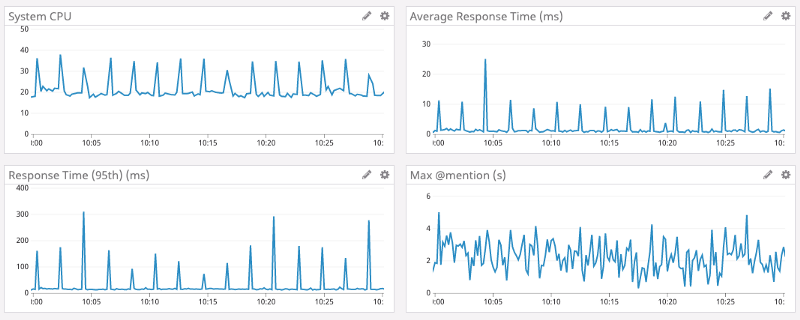
\includegraphics[width=\textwidth,height=\textheight,keepaspectratio]{images/discord-spikes.png}

\end{frame}

% ----------------------------------------------------------------- %

\begin{frame}
\frametitle{Why companies sometimes do \textbf{not} use Rust?}

\begin{itemize}
    \item Already wrote a lot of code in another language
    \item Company's internal tools do not support Rust, and maintenance could be costly
    \item In a big company, you should have your committee to help support language in the company.
    \item Hard to find developers in such a difficult and fresh language
    \item Rust developers are usually talented people with high salary expectations
\end{itemize}
\end{frame}

% ----------------------------------------------------------------- %


\begin{frame}[fragile]
\frametitle{But why are we learning Rust?}
\textbf{CVE-2008-0166}

Bug in \texttt{glibc} that resulted in vulnerability in OpenSSL.

\begin{itemize}
    \item \texttt{srandom()} - set seed for non-cryptographic pseudorandom number generator.
    \item If read from \texttt{/dev/random} failed, the following code is executed:
\end{itemize}

\begin{minted}{C}
  struct timeval tv;
  unsigned long junk;
  gettimeofday(&tv, NULL);
  srandom((getpid() << 16) ^ tv.tv_sec ^ tv.tv_usec ^ junk);
\end{minted}

\end{frame}

% ----------------------------------------------------------------- %

\begin{frame}[fragile]
\frametitle{UB example}
\textbf{CVE-2008-0166}

Bug in \texttt{glibc} that resulted in vulnerability in OpenSSL.

\begin{itemize}
    \item \texttt{srandom()} - set seed for non-cryptographic pseudorandom number generator.
    \item If read from \texttt{/dev/random} failed, the following code is executed:
\end{itemize}

\begin{minted}{C}
  struct timeval tv;
  unsigned long junk;
  gettimeofday(&tv, NULL);
  srandom(junk);
\end{minted}

One day, the compiler decided to remove everything except junk :D

\end{frame}


% ----------------------------------------------------------------- %

\begin{frame}[fragile]
\frametitle{But why are we learning Rust?}

\begin{minted}{C}
  Vec* vec_new() {
      Vec vec;
      vec.data = NULL;
      vec.length = 0;
      vec.capacity = 0;
      return &vec;
  }
\end{minted}

\end{frame}


% ----------------------------------------------------------------- %

\begin{frame}[fragile]
\frametitle{Dangling pointer}

\begin{minted}{C}
  Vec* vec_new() {
      Vec vec;
      vec.data = NULL;
      vec.length = 0;
      vec.capacity = 0;
      return &vec; // returning a reference to a local var
  }
\end{minted}

\end{frame}

% ----------------------------------------------------------------- %

\begin{frame}[fragile]
\frametitle{But why are we learning Rust?}

\begin{minted}{C}
  void main() {
      Vec *vec = vec_new();

      /* ... */

      free(vec->data);
      vec_free(vec);
  }
\end{minted}

\end{frame}

% ----------------------------------------------------------------- %

\begin{frame}[fragile]
\frametitle{Double free}

\begin{minted}{C}
  void main() {
      Vec *vec = vec_new();

      /* ... */

      free(vec->data);
      vec_free(vec); // double free
  }
\end{minted}

\end{frame}

% ----------------------------------------------------------------- %

\begin{frame}[fragile]
\frametitle{But why are we learning Rust?}

\begin{minted}{C}
  void main() {
      /* ... */

      int *n = &vec->data[0];
      vec_push(vec, 110);
      printf("%d\n", *n);

      /* ... */
  }
\end{minted}

\end{frame}

% ----------------------------------------------------------------- %

\begin{frame}[fragile]
\frametitle{Iterator Invalidation}

\begin{minted}{C}
  void main() {
      /* ... */

      int *n = &vec->data[0];
      vec_push(vec, 110); // may be reallocation
      printf("%d\n", *n);

      /* ... */
  }
\end{minted}

\end{frame}

% ----------------------------------------------------------------- %

\begin{frame}[c]
\frametitle{C\texttt{++} problems}
What is common?
\begin{itemize}
    \item UB
    \item Double free
    \item Dangling pointer
    \item Iterator invalidation
\end{itemize}
\end{frame}

% ----------------------------------------------------------------- %

\begin{frame}[fragile]
\frametitle{Is Rust safe?}
Rust is theoretically proven to be safe.\\

\begin{tabular}{cl}  
\begin{tabular}{c}
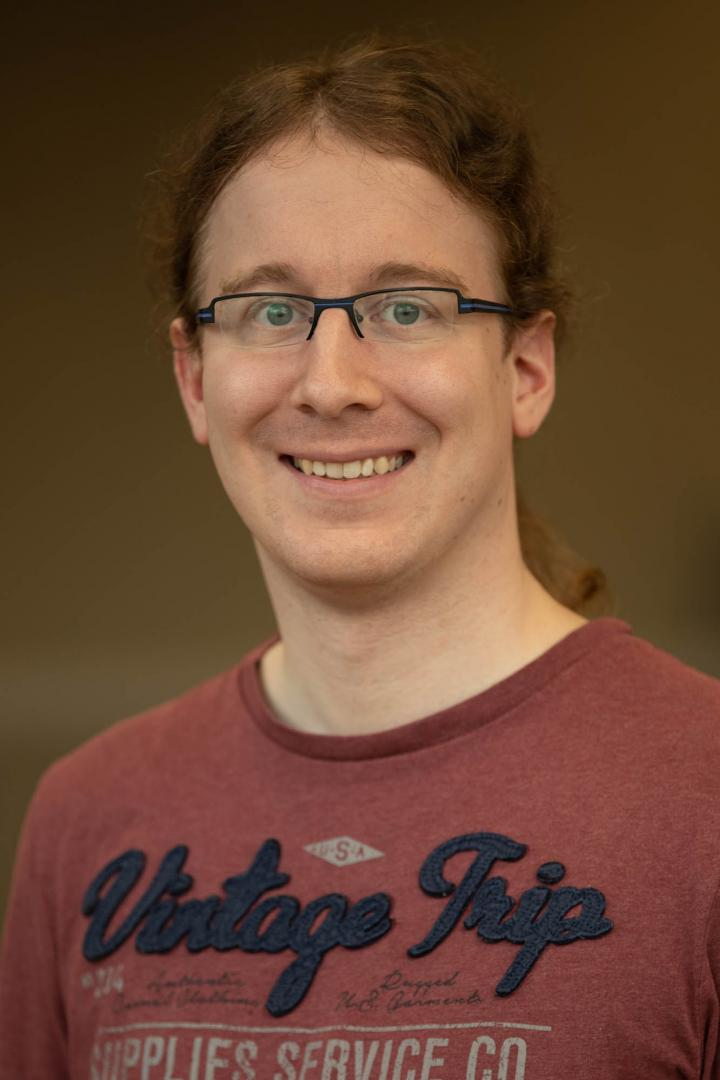
\includegraphics[height=5cm, width=3.5cm]{images/ralf-jung.jpeg}
\end{tabular}
& \begin{tabular}{l}
\parbox{0.5\linewidth}{
    \href{https://www.ralfj.de/research/thesis.html}{Understanding and Evolving the Rust Programming Language, Ralf Jung, August 2020.}

    Awards:
    \begin{itemize}
        \item 2021 Otto Hahn Medal
        \item Honorable Mention for the 2020 ACM Doctoral Dissertation Award
        \item 2021 ETAPS Doctoral Dissertation Award
    \end{itemize}
}
\end{tabular}  \\
\end{tabular}
\end{frame}

% ----------------------------------------------------------------- %

\begin{frame}[fragile]
\frametitle{Is Rust safe?}
RustBelt - formal model of Rust that includes core conceptions of language (borrowing, lifetimes, lifetime inclusion).

\begin{itemize}
    \item Proof of safety of Safe\footnote{There exists Unsafe Rust, but we will return to it later.} Rust
    \item Definition of sufficiency conditions for every type \texttt{T} to consider it safe abstraction
    \item Proof of soundness (no UB or Memory unsafety): \texttt{Cell}, \texttt{RefCell}, \texttt{thread::spawn}, \texttt{Mutex}, \texttt{RwLock}, \texttt{Arc}, \dots
\end{itemize}
\end{frame}

% ----------------------------------------------------------------- %

\begin{frame}
\frametitle{Rust pros summary}
\textbf{Rust language}

Pros:
\begin{itemize}
    \item Don't require any runtime
    \item Provides a thick layer of abstraction, allowing to write complex readable code: structures, generics, traits, closures, iterators...
    \item \textbf{No memory unsafety and undefined behavior}\footnote{Unless you or your dependencies use \texttt{unsafe} incorrectly}
    \item Modern standard without any\footnote{There exist not good decisions.} incorrect decisions
\end{itemize}

According to \href{https://www.zdnet.com/article/microsoft-70-percent-of-all-security-bugs-are-memory-safety-issues/}{Microsoft} and \href{https://www.chromium.org/Home/chromium-security/memory-safety}{Chromium}, ~70\% of bugs involve memory unsafety.
\end{frame}

% ----------------------------------------------------------------- %

\begin{frame}[c]
\centering\Huge\textbf{Finally some Rust}
\end{frame}

% ----------------------------------------------------------------- %

\begin{frame}[fragile]
\frametitle{Hello, World!}

How to write Hello World in Rust?

\begin{minted}{rust}
    fn main() {
        println!("Hello, World!");
    }
\end{minted}
\end{frame}

% ----------------------------------------------------------------- %

\begin{frame}[fragile]
\frametitle{Hello, World!}

How to write Hello World in Rust?

\begin{minted}{rust}
    fn main() {
        println!("Hello, World!");
    }
\end{minted}

\begin{minted}{bash}
    $ rustc main.rs  # no optimizations
    $ ./main
    Hello, World!
\end{minted}
\end{frame}

% ----------------------------------------------------------------- %


\begin{frame}[fragile]
\frametitle{Hello, World!}

How to write Hello World in Rust: assembly edition.

\begin{minted}[fontsize=\small]{rust}
    #![no_main]

    #[link_section=".text"]
    #[no_mangle]
    pub static main: [u32; 9] = [
        3237986353,
        3355442993,
        120950088,
        822083584,
        252621522,
        1699267333,
        745499756,
        1919899424,
        169960556,
    ];
\end{minted}
\end{frame}

% ----------------------------------------------------------------- %

\begin{frame}[fragile]
\frametitle{Defining variables}
\textbf{Integer variable types:}

\begin{table}[]
\begin{tabular}{|l|l|l|l|l|l|l|}
\hline
Bits count & 8  & 16  & 32  & 64  & 128  & 32/64 \\ \hline
Signed     & \texttt{i8} & \texttt{i16} & \texttt{i32} & \texttt{i64} & \texttt{i128} & \texttt{isize} \\ \hline
Unsigned   & \texttt{u8} & \texttt{u16} & \texttt{u32} & \texttt{u64} & \texttt{u128} & \texttt{usize} \\ \hline
\end{tabular}
\end{table}

\texttt{usize} - size of the pointer.
\end{frame}

% ----------------------------------------------------------------- %

\begin{frame}[fragile]
\frametitle{Defining variables}
To define a variable, use \texttt{let} keyword:

\begin{minted}{rust}
    let idx: usize = 42;
\end{minted}

Literals:

\begin{minted}{rust}
    let y = 92_000_000i64;
    let hex_octal_bin = 0xffff_ffff + 0o777 + 0b1;
\end{minted}

In Rust there's \textbf{type inference}. For integer type, the default type is \texttt{i32}.

\begin{minted}{rust}
    let idx = 42;
\end{minted}

Variables are \textbf{immutable} by default. To make a variable mutable, use \texttt{mut} keyword:

\begin{minted}{rust}
    let mut idx: usize = 0x1022022;
\end{minted}
\end{frame}

% ----------------------------------------------------------------- %

\begin{frame}[fragile]
\frametitle{Compiled?}

\begin{minted}{rust}
    fn main() {
        let x: i32 = 42;
        let y = 4;
        
        x = y + 1;
    }
\end{minted}

\end{frame}

% ----------------------------------------------------------------- %

\begin{frame}[fragile]
\frametitle{Compiled?}

\begin{minted}{rust}
    fn main() {
        let x: i32 = 42;
        let y = 4;
        
        x = y + 1;
    }
\end{minted}

No :(

\end{frame}

% ----------------------------------------------------------------- %

\begin{frame}[fragile]
\frametitle{Bool}

In Rust, \texttt{bool} can have only two values: \texttt{true} and \texttt{false}:

\begin{minted}{rust}
    let mut x = true;
    x = false;
    x = 1; 
\end{minted}

\end{frame}

% ----------------------------------------------------------------- %

\begin{frame}[fragile]
\frametitle{Bool}

In Rust, \texttt{bool} can have only two values: \texttt{true} and \texttt{false}:

\begin{minted}{rust}
    let mut x = true;
    x = false;
    x = 1; // error: expected `bool`, found integer!
\end{minted}

At the same time, it's 1 byte in memory (will be important later).

\end{frame}

% ----------------------------------------------------------------- %

\begin{frame}[fragile]
\frametitle{Bool}
\begin{minted}{rust}
    let to_be = true;
    let not_to_be = !to_be;
    let the_question = to_be || not_to_be;
\end{minted}

\texttt{\&\&} and \texttt{||} are lazy.
\end{frame}

% ----------------------------------------------------------------- %

\begin{frame}[fragile]
\frametitle{Arithmetic}
\begin{itemize}
    \item Basic arithmetic: \texttt{+}, \texttt{-}, \texttt{*}, \texttt{/}, \texttt{\%}
    \item \texttt{/}, \texttt{\%} round to 0.
\begin{minted}{rust}
    let (x, y) = (15, -15);
    let (a1, b1) = (x / -4, x % -4);
    let (a2, b2) = (y /  4, y %  4);

    println!("{a1} {b1} and {a2} {b2}");
    // outputs "-3 3 and -3 -3"
\end{minted}
    \item No \texttt{++}
    \item Bitwise and logical operations \texttt{!}, \texttt{<<}, \texttt{>>}, \texttt{|}, \texttt{\&}
    \item \href{https://doc.rust-lang.org/book/appendix-02-operators.html}{Full list of operators here}
\end{itemize}
\end{frame}

% ----------------------------------------------------------------- %

\begin{frame}[fragile]
\frametitle{Type casting}
In Rust, there's no type implicit casting:

\begin{minted}[fontsize=\small]{rust}
    let x: u16 = 1;
    let y: u32 = x; // error: mismatched types 

    
    let a: u32 = x as u16;
    let b: u32 = x.into();

    let x: i64 = 1;
    let y: i32 = x as i32; // working
    let y: i32 = x.into(); // not working
\end{minted}

\texttt{as} - explicit casting operator \newline
\texttt{into} - trait
\end{frame}

% ----------------------------------------------------------------- %

\begin{frame}[fragile]
\frametitle{Type casting}
\textbf{Note}: Casting is not transitive, that is, even if:

\begin{minted}{rust}
    e as U1 as U2
\end{minted}

Is a valid expression, the expression:

\begin{minted}{rust}
    e as U2
\end{minted}

It is not necessarily so.
\end{frame}

% ----------------------------------------------------------------- %

\begin{frame}[fragile]
\frametitle{Overflow}
Overflow is a programmer's mistake. In debug build vs in release build:

\begin{minted}[fontsize=\small]{rust}
    fn main() {
        let x = i32::MAX;
        let y = x + 1;
        println!("{}", y);
    }
\end{minted}

\begin{minted}[fontsize=\small]{bash}
    $ cargo run
    thread 'main' panicked at 'attempt to add with overflow',
    main.rs:3:13

    $ cargo run --release
    -2147483648
\end{minted}
\end{frame}


% ----------------------------------------------------------------- %

\begin{frame}[fragile]
\frametitle{Explicit arithmetic}
\begin{minted}[fontsize=\small]{rust}
    let x = i32::MAX;

    let y = x.wrapping_add(1);
    assert_eq!(y, i32::MIN);

    let y = x.saturating_add(1);
    assert_eq!(y, i32::MAX);

    let (y, overflowed) = x.overflowing_add(1);
    assert!(overflowed);
    assert_eq!(y, i32::MAX)

    match x.checked_add(1) {
        Some(y) => unreachable!(),
        None => println!("overflowed"),
    }
\end{minted}
\end{frame}

% ----------------------------------------------------------------- %

\begin{frame}[fragile]
\frametitle{Floating point}
\begin{minted}{rust}
    let y = 0.0f32; // Litaral f32
    let x = 0.0;    // Default value (f64)

    // let z: f32 = 0;
    // Point is necessary
    // error: expected f32, found integer variable
    
    let z = 0.0f32;

    let not_a_number = std::f32::NAN;
    let inf = std::f32::INFINITY;

    // Wow, so many functions!
    8.5f32.ceil().sin().round().sqrt()
\end{minted}
\end{frame}

% ----------------------------------------------------------------- %

\begin{frame}[fragile]
\frametitle{Prelude}
Default includes:
\begin{itemize}
    \item \begin{minted}{rust}
std::vec::Vec
    \end{minted}
    \item \begin{minted}{rust}
std::string::{String, ToString}
    \end{minted}
    \item \begin{minted}{rust}
std::option::Option::{self, Some, None}
    \end{minted}
    \item \href{https://doc.rust-lang.org/std/prelude/index.html#the-rust-prelude}{And others...}
\end{itemize}

Turning off:
\begin{minted}{rust}
    #![no_implicit_prelude]    
\end{minted}
\end{frame}

% ----------------------------------------------------------------- %

\begin{frame}[fragile]
\frametitle{Tuple}
\begin{minted}[fontsize=\small]{rust}
    let pair: (f32, i32) = (0.0, 92);
    let (x, y) = pair;
    // The same as this
    // Note the shadowing!
    let x = pair.0;
    let y = pair.1;

    let void_result = println!("hello");
    assert_eq!(void_result, ());

    let trailing_comma = (
        "Archibald",
        "Buttle",
    );
\end{minted}
\end{frame}

% ----------------------------------------------------------------- %

\begin{frame}[fragile]
\frametitle{Tuple}
\begin{minted}{rust}
    // Zero element tuple, or Unit
    let x = ();
    let y = {};
    assert!(x == y); // OK

    // One element tuple
    let x = (42,);
\end{minted}
\end{frame}

% ----------------------------------------------------------------- %

\begin{frame}[fragile]
\frametitle{Tuple}
In memory, tuple is stored continuously.

\begin{table}[]
\begin{tabular}{|l|l|}
\hline
\texttt{7}        & \texttt{07 00 00 00}             \\ \hline
\texttt{(7, 263)} & \texttt{07 00 00 00 07 01 00 00} \\ \hline
\end{tabular}
\end{table}
\end{frame}

% ----------------------------------------------------------------- %

\begin{frame}[fragile]
\frametitle{Tuple}
Tuple is a zero-cost abstraction!

\begin{minted}{rust}
    let t = (92,);
    // 0x7ffc6b2f6aa4
    println!("{:?}", &t as *const (i32,));
    // 0x7ffc6b2f6aa4
    println!("{:?}", &t.0 as *const i32);
\end{minted}

Meanwhile in Python:

\begin{minted}{py}
    t = (92,)
    print(id(t))     # 139736506707248
    print(id(t[0]))  # 139736504680928
\end{minted}
\end{frame}

% ----------------------------------------------------------------- %

\begin{frame}[fragile]
\frametitle{More on shadowing}
What is the output of this code?

\begin{minted}{rust}
    let x = 10;
    for i in 0..5 {
        if x == 10 {
            println!("{i} {x}");
            let x = 12;
        }
    }
\end{minted}
\end{frame}

% ----------------------------------------------------------------- %

\begin{frame}[fragile]
\frametitle{More on shadowing}
What is the output of this code?

\begin{minted}{rust}
    let x = 10;
    for i in 0..5 {
        if x == 10 {
            println!("{i} {x}");
            let x = 12;
        }
    }
    // This code outputs 0 10\n1 10\n2 10\n3 10\n4 10\n
\end{minted}
\end{frame}

% ----------------------------------------------------------------- %

\begin{frame}[fragile]
\frametitle{More on shadowing}
Drop is compiler optimization. \href{https://rust.godbolt.org/z/3b5hfr7db}{Godbolt}.

\begin{minted}{rust}
    pub fn shadowing(num: i32) -> i32 {
        let vec = vec![0, 1, 2, 3];
        let vec = vec![4, 5, 6, 7];
        vec[0]
    }
\end{minted}
\end{frame}

% ----------------------------------------------------------------- %

\begin{frame}[fragile]
\frametitle{Array}
\begin{minted}{rust}
    let xs: [u8; 3] = [1, 2, 3];
    assert_eq!(xs[0], 1);    // index -- usize
    assert_eq!(xs.len(), 3); // len() -- usize

    let mut buf = [0u8; 1024];
\end{minted}

The size of an array is a constant known at compile-time and the part of the type.
\end{frame}

% ----------------------------------------------------------------- %

\begin{frame}[fragile]
\frametitle{References}
\begin{itemize}
    \item Is really a pointer in compiled program.
    \item Cannot be \texttt{NULL}.
    \item Guaranties that the object is alive.
    \item There are \textt{\&} and \textt{\&mut} references.
\end{itemize}

\begin{minted}{rust}
    let mut x: i32 = 92;
    let r: &mut i32 = &mut x;  // Reference created explicitly
    *r += 1;                   // Explicit dereference
\end{minted}
\end{frame}

% ----------------------------------------------------------------- %

\begin{frame}[fragile]
\frametitle{References}
In C\texttt{++} we have to use \texttt{std::reference\_wrapper} to store a reference in a vector:

\begin{minted}{cpp}
    int x = 10;
    std::vector<std::reference_wrapper<int>> v;
    v.push_back(x);
\end{minted}

In Rust, references are a first class objects so we can push them to vector directly:

\begin{minted}{rust}
    let x = 10;
    let mut v = Vec::new();
    v.push(&x);
\end{minted}
\end{frame}

% ----------------------------------------------------------------- %

\begin{frame}[fragile]
\frametitle{Pointers}
\begin{itemize}
    \item Useless without \textt{unsafe}, because you cannot dereference it.
    \item Can be NULL.
    \item Does not guarrantee that the object is alive.
    \item \textbf{Very rarely needed}. Examples: FFI, some data structures, optimizations...
\end{itemize}

\begin{minted}{rust}
    let x: *const i32 = std::ptr::null();
    let mut y: *const i32 = std::ptr::null();
    let z: *mut i32 = std::ptr::null_mut();
    let mut t: *mut i32 = std::ptr::null_mut();
\end{minted}

In Rust, we read type names from left to right, not from right to left like in C++:

\begin{minted}{cpp}
    uint32_t const * const x = nullptr;
    uint32_t const * y = nullptr;
    uint32_t* const z = nullptr;
    uint32_t* t = nullptr;
\end{minted}
\end{frame}

% ----------------------------------------------------------------- %

\begin{frame}[fragile]
\frametitle{Box}
\begin{itemize}
    \item Pointer to some data on the heap.
    \item Pretty like C\texttt{++}'s \texttt{std::unique\_ptr}, but without \texttt{NULL}
\end{itemize}

\begin{minted}{rust}
    let x: Box<i32> = Box::new(92);
\end{minted}
\end{frame}

% ----------------------------------------------------------------- %

\begin{frame}[fragile]
\frametitle{Functions}
Functions are defined via \texttt{fn} keyword. Note the expressions and statements!

\begin{minted}[fontsize=\small]{rust}
    fn func1() {}
    fn func2() -> () {}
    fn func3() -> i32 {
        0
    }
    fn func4(x: u32) -> u32 {
        return x;
    }
    fn func5(x: u32, mut y: u64) -> u64 {
        y = x as u64 + 10;
        return y
    }
    fn func6(x: u32, mut y: u64) -> u32 {
        x + 10
    }
\end{minted}
\end{frame}

% ----------------------------------------------------------------- %

\begin{frame}
\frametitle{Summary}
\begin{itemize}
    \item Motivation
    \item Basic syntax
    \item Primitive types
\end{itemize}
\end{frame}

% ----------------------------------------------------------------- %

\begin{frame}
\frametitle{Questions?}
\begin{center}

\includegraphics[width=\textwidth,height=7cm,keepaspectratio]{images/crab.jpg}
\end{center}
\end{frame}

% ----------------------------------------------------------------- %

\end{document}
